\documentclass[11pt]{article}
\usepackage{enumitem}
\usepackage[margin=1in]{geometry}
\usepackage{graphicx}
\usepackage[space]{grffile}
\usepackage{adjustbox}

\author{Zipeng Fu}
\date{\today}
\title{CSM164 Homework 1}

\begin{document}
\maketitle
\newpage

\section{Splitting Heuristic for Decision Trees}
\begin{enumerate}[label=(\alph*)]
    \item
        The best 1-leaf decision tree making minimum error should output 1 for all instance examples. Hence, the mistakes made should be total number times the probability of examples with label $Y = 0$.

        $$2^n * \left(\frac{1}{2}\right)^3 = 2^{n-3}$$

    \item
        No, there is no such split. If the split is based on $X_i$ where $i\geq4$, the output of both branches should be 1, because $\frac{7}{8}$ of probability is $Y = 1$. Thus, this split is trivial and make no difference from the case in part (a). For $i\leq3$, when $X_i$ is 1, the output should be 1 due to the disjunctive relation. For $X_i$ is 0, the probability $Y=1$ given $X_i = 0$ is
        $$\left(\frac{1}{2}+\frac{1}{2}\right)-\frac{1}{2}*\frac{1}{2}=\frac{3}{4}.$$
        The result is larger than $Y=0$ given $X_i = 0$, so the predicted output should still be 1. And the overall number of mistakes made is
        $$\left[\left(1-\frac{3}{4}\right)*\frac{1}{2}\right]*2^{n} = \frac{1}{8}*2^{n} = 2^{n-3},$$
        which is the same as the result in part (a).
    
    \item
        $$\mathrm{Entropy} = -\frac{1}{8}*\log_2{\left(\frac{1}{8}\right)} - \frac{7}{8}*\log_2{\left(\frac{7}{8}\right)} \approx 0.54356$$
    
    \item
        Yes, the method in part (b) reduces the entropy of the output $Y$. The conditional entropy is $$\mathrm{Entropy} = \frac{1}{2} \left(-\frac{3}{4}\log_2{\left(\frac{3}{4}\right)} - \frac{1}{4}\log_2{\left(\frac{1}{4}\right)}\right) + \frac{1}{2}*0 \approx 0.40564. $$
        $$\mathrm{Information\:Gain} \approx 0.54356 - 0.40564 = 0.13792$$
\\
\end{enumerate}


\section{Entropy and INformation}
\begin{enumerate}[label=(\alph*)]
    \item
        If the ratio $\frac{p_k}{p_k+n_k}$ is the same for all k, then the fraction of positive for the superset $X_i$ is also the same. Let the ratio be $r$.
        $$H\left(\mathrm{S\_before\_split}\right) = B\left(r\right)$$
        $$H\left(\mathrm{S\_after\_split}\right) = \sum_{i=0}^{k}{\mathrm{fraction}\left(S_i\right)H\left(S_i\right)} = \sum_{i=0}^{k}{\mathrm{fraction}\left(S_i\right)B\left(r\right)} = \left[\sum_{i=0}^{k}{\mathrm{fraction}\left(S_i\right)}\right] * B\left(r\right) = B\left(r\right)$$
        Hence, the entropies before the split and after the split are equal, which means the information gain of this attribute is 0.
\\
\end{enumerate}

\section{k-Nearest Neighbors and Cross-validation}
\begin{enumerate}[label=(\alph*)]
    \item
        When k is 1, the nearest neighbor is the testing point itself, selecting from the training set. Thus, no error will occur and the minimum resulting trainning error is 0.\\
    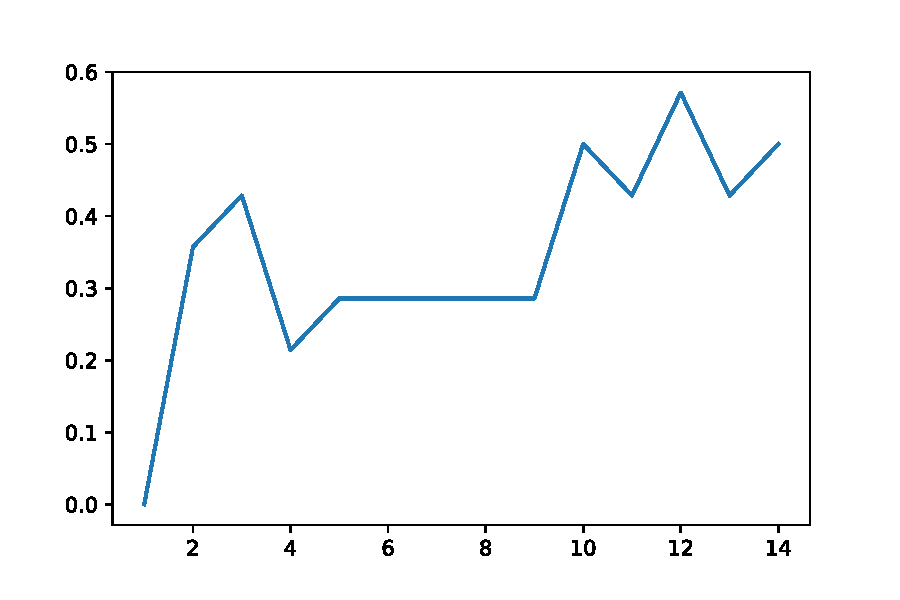
\includegraphics{3aGraph.pdf}
    \begin{verbatim}
    from sklearn.neighbors import KNeighborsClassifier as KNN
    import matplotlib.pyplot as plt
    X = [[1,5],[2,6],[2,7],[3,7],[3,8],[4,8],[5,1],[5,9],\
        [6,2],[7,2],[7,3],[8,3],[8,4],[9,5]]
    y = [0, 0, 1, 0, 1, 0, 1, 0, 1, 0, 1, 0, 1, 1]
    klist = []
    errlist = []
    for k in range(1, 15):
        knn = KNN(n_neighbors=k, p=2)
        knn.fit(X, y)
        errCount = 0
        predict = knn.predict(X)
        for i in range(14):
            if predict[i] != y[i]:
                errCount += 1
        klist.append(k)
        errlist.append(errCount/14)
    plt.plot(klist, errlist)
    plt.savefig("3aGraph.svg")
    \end{verbatim}

    \item
        For KNN problems, the choice of the hyper-parameter, k, is crucial. Using too large values k will make distinctions between difference classes blurred. The label predicted largely relies on the global majority labels in the training set, instead of the local majority. On the other hand, too small values of k will let the predicted labels of test set susceptible to noise in the training set. The results are prone to outliners near the test input attribute values (Detailed graph plot is shown in part a).

    \item
        When k equals to 5 or 7, the leave-one-out cross-validation error is minimized. The resulting error is 4 out of 14 test examples (0.285714285).\\
    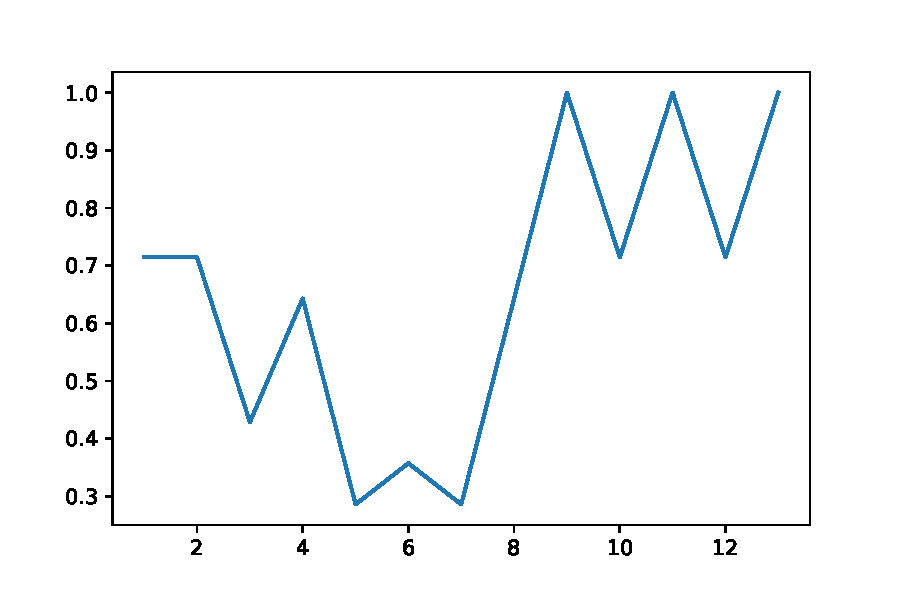
\includegraphics{3cGraph.pdf}
    \begin{verbatim}
    from sklearn.neighbors import KNeighborsClassifier as KNN
    import matplotlib.pyplot as plt
    X = [[1,5],[2,6],[2,7],[3,7],[3,8],[4,8],[5,1],\
        [5,9],[6,2],[7,2],[7,3],[8,3],[8,4],[9,5]]
    y = [0, 0, 1, 0, 1, 0, 1, 0, 1, 0, 1, 0, 1, 1]
    klist = []
    errlist = []
    for k in range(1, 14):
        errCount = 0
        for i in range(14):
            knn = KNN(n_neighbors=k, p=2)
            knn.fit(X[:i]+X[i+1:], y[:i]+y[i+1:])
            predict = knn.predict([X[i]])
            if predict[0] != y[i]:
                errCount += 1
        klist.append(k)
        errlist.append(errCount/14)
    plt.plot(klist, errlist)
    plt.savefig("3cGraph.pdf")
    \end{verbatim}
\end{enumerate}


\section{Programming exercise: Applying decision trees and k-nearest neighbors}
\begin{enumerate}[label=(\alph*)]
    \item
    \adjustbox{valign=t}{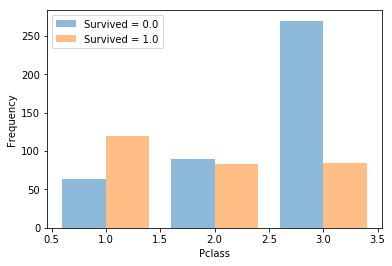
\includegraphics[width=0.3\textwidth]{download.png}}
    \adjustbox{valign=t}{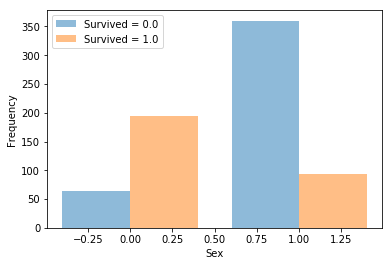
\includegraphics[width=0.3\textwidth]{download (1).png}}
    \adjustbox{valign=t}{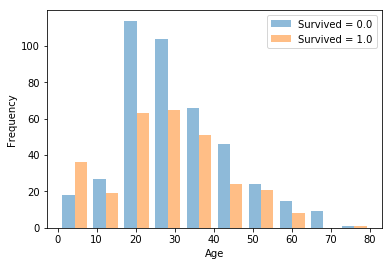
\includegraphics[width=0.3\textwidth]{download (2).png}}\\
    \adjustbox{valign=t}{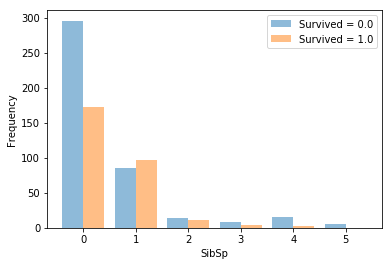
\includegraphics[width=0.3\textwidth]{download (3).png}}
    \adjustbox{valign=t}{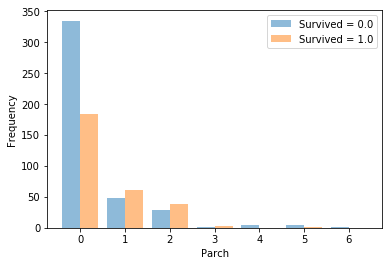
\includegraphics[width=0.3\textwidth]{download (4).png}}
    \adjustbox{valign=t}{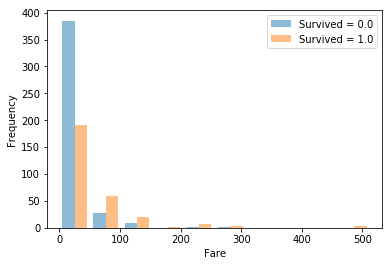
\includegraphics[width=0.3\textwidth]{download (5).png}}\\
    \adjustbox{valign=t}{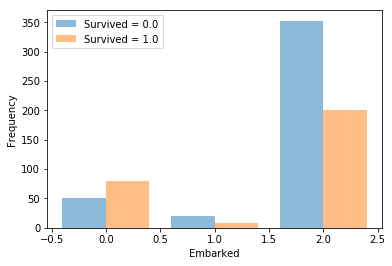
\includegraphics[width=0.3\textwidth]{download (6).png}}
    \begin{enumerate}
        \item[Ticket Class] Upper class passengers tend to have a higher survival rate than lower classes.
        \item[Sex] Women tend to have a higher survival rate than men.
        \item[Age] Young kids below 10 years old and the eldly over 70 years old have a higher survival rate than teenagers, young adults and middle-aged adults.
        \item[Siblings/Spouses] People with 1 sibling or spouse have a higher survival rate than any other groups.
        \item[Parents/Children] People with no parents or children have a significant lower survival rate than other groups.
        \item[Fare] People paying less than \$50 have the lowest survival rate. Other groups survived with approximately same percentage.
        \item[Port Embark] (0 = Cherbourg, 1 = Queenstown, 2 = Southampton) People embarked in Chengbourg have the lowest survival rate. The other 2 groups have approximately same survival rate.
    \end{enumerate}

    \item
    RandomClassifier have a property of probability. I set it to be the probability of 0 as the predicted label. Since the seed is fixed, the pseudo-random number generator will generate the same sequence of 0 and 1 with corresponding probabilities. Hence, the resulting error is fixed, which is 0.485.
    \begin{verbatim}
Classifying using Random...
-- training error: 0.485
    \end{verbatim}

    \item
    Set the decision tree model to be based on information gain by passing in the parameter, $criterion$, to be $entropy$. Training error of this Dicision Tree Classifier based on information gain is 0.014.
    \begin{verbatim}
Classifying using Decision Tree...
-- training error: 0.014
    \end{verbatim} 

    \item
    I set the parameter of $KNeighborsClassifier$, $n\_neighbors$, to be 3, 5, 7, respectively. Euclidean distance is used, $p = 2$. The results are
    \begin{verbatim}
Classifying using k-Nearest Neighbors...
-- training error: 0.167 when k = 3
-- training error: 0.201 when k = 5
-- training error: 0.240 when k = 7.
    \end{verbatim}

    \item 
    I set the $random\_state$ of $train\_test\_split$ to be from 0 to 99. Then the pseudo number sequence is unchanged during each execution, so the output averages are fixed. The result is not normalized, as indicated on Piazza.
    \begin{verbatim}
Investigating various classifiers...
Average results of MajorityVoteClassifier:
-- training error: 0.404, test error: 0.407
Average results of RandomClassifier:
-- training error: 0.489, test error: 0.487
Average results of DecisionTreeClassifier:
-- training error: 0.012, test error: 0.241
Average results of KNeighborsClassifier:
-- training error: 0.212, test error: 0.315
    \end{verbatim}
    \newpage

    \item
    (The features are not normalized.) In the figure below, the vertical axis is the validation error rate and the horizontal axis is the odd number, k. As we can see, the best value of k is 7, given the lowest error rate of 7 Nearest-Neighbors Model.
    \\
    \adjustbox{center}{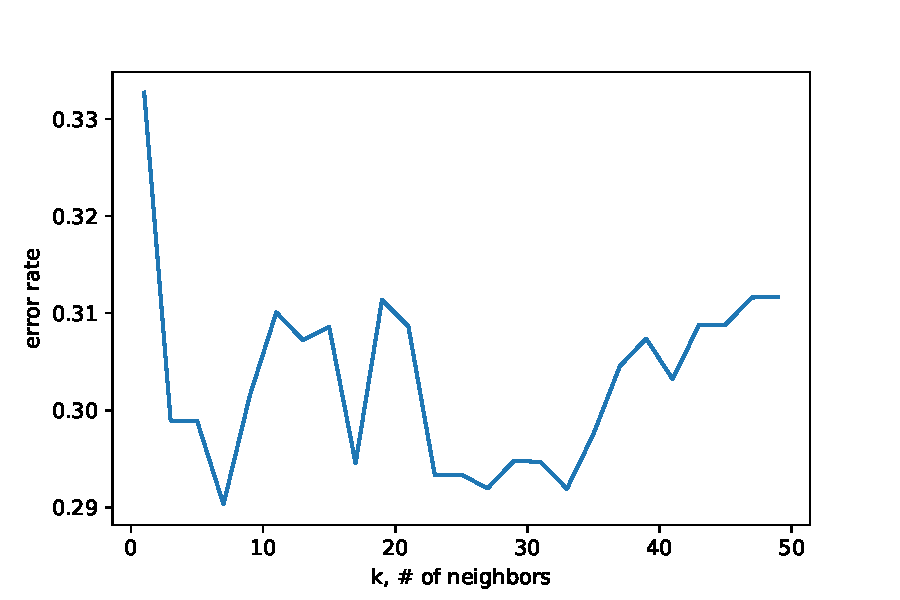
\includegraphics{4fGraph.pdf}}
    \newpage

    \item 
    The best depth limit to use for this dataset is 3, where the test error is the lowest, which is just above 0.20. As we can observe from the graph, the overfiting occurs after the depth limit exceeds 3, because the test error starts to show an increasing trend when depth limit is more than 3, and at the same time, the training error keeps decreasing. This is the phenomenon of overfitting, which can be regularized by limiting the maximum depth based on validation set results.
    \\
    \adjustbox{valign=t}{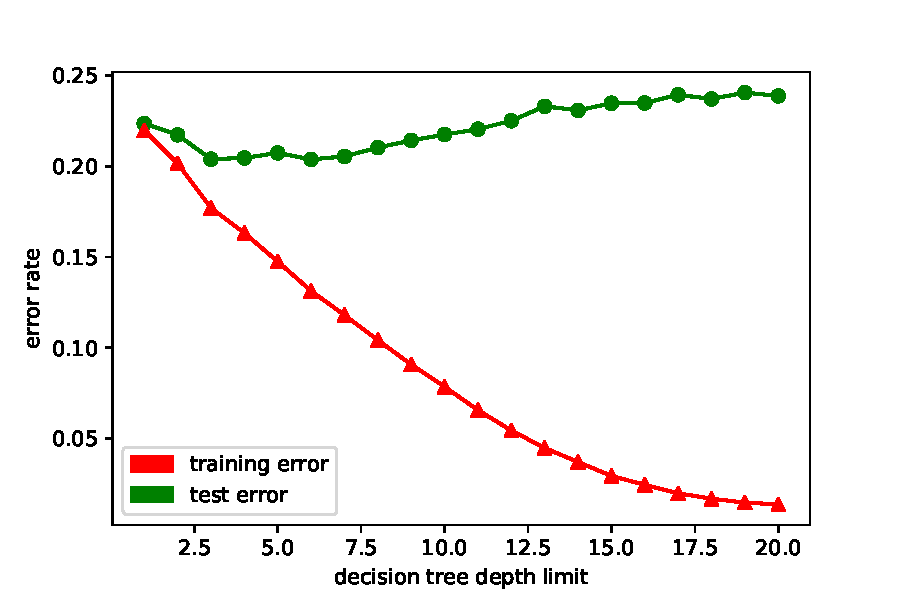
\includegraphics{4gGraph.pdf}}
    \newpage

    \item
    The upper graph is the results of one-time computation based on random splits of training set with designated portions. The lower graph is the results of average error rates of 100 random splits (with different $random\_state$) for each designated portions of training set from 0.1 to 1.0. All test errors are calculated given the same test set. As we can see, the fluctuations in upper graph indicates the bias in extracted training sets, I made the second graph to mitigate biases. DT training error shows an increasing trend before 0.5, possibly due to our aim to minimize entropy instread of error rate, as discuss in Question 1. Both test errors of DT and KNN show the decreasing trend. Slight increases after 0.7/0.8 may be caused by overfitting. Because of lack of feature normalization, feature selection to avoid the curse of high dimension and methods to convert categorial data (eg. embark ports) to numerial data, the incoming data are noisy and the training errors of KNN stay high despite increasing amount of training data. For this data set, Decision Tree has a better performance than KNN model.
    \\
    \adjustbox{center}{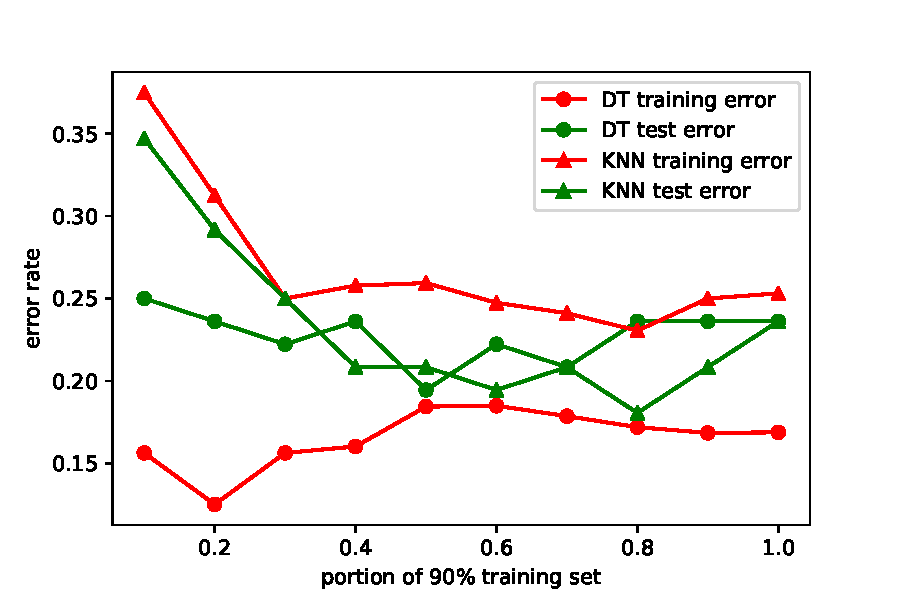
\includegraphics[width=0.5\paperwidth]{4hGraph.pdf}}\\
    \adjustbox{center}{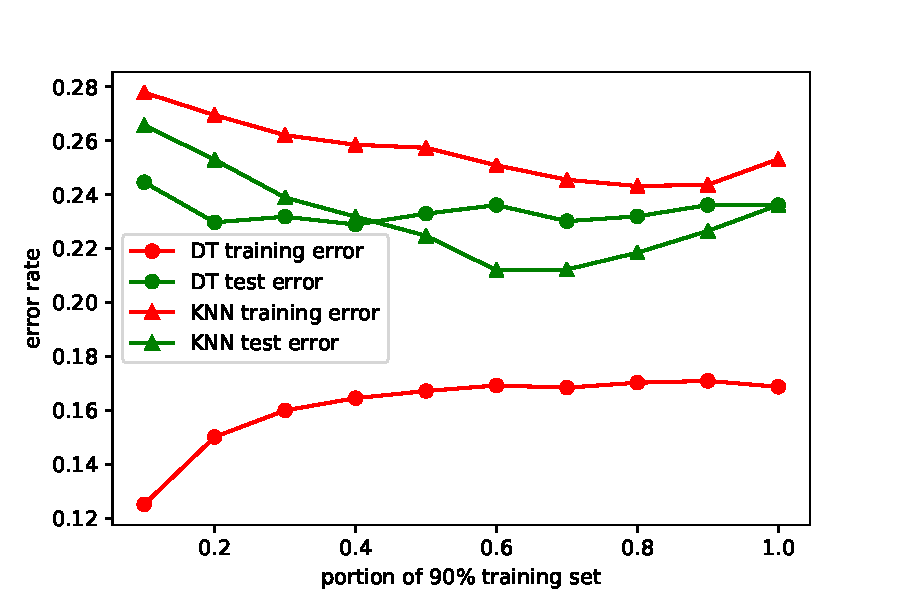
\includegraphics[width=0.5\paperwidth]{4hGraph2.pdf}}\\




\end{enumerate}




\end{document}